% C9. Kaggle frente a negocio
\begin{frame}{Lo que gana en Kaggle no es lo que gana la empresa}
  \centering
  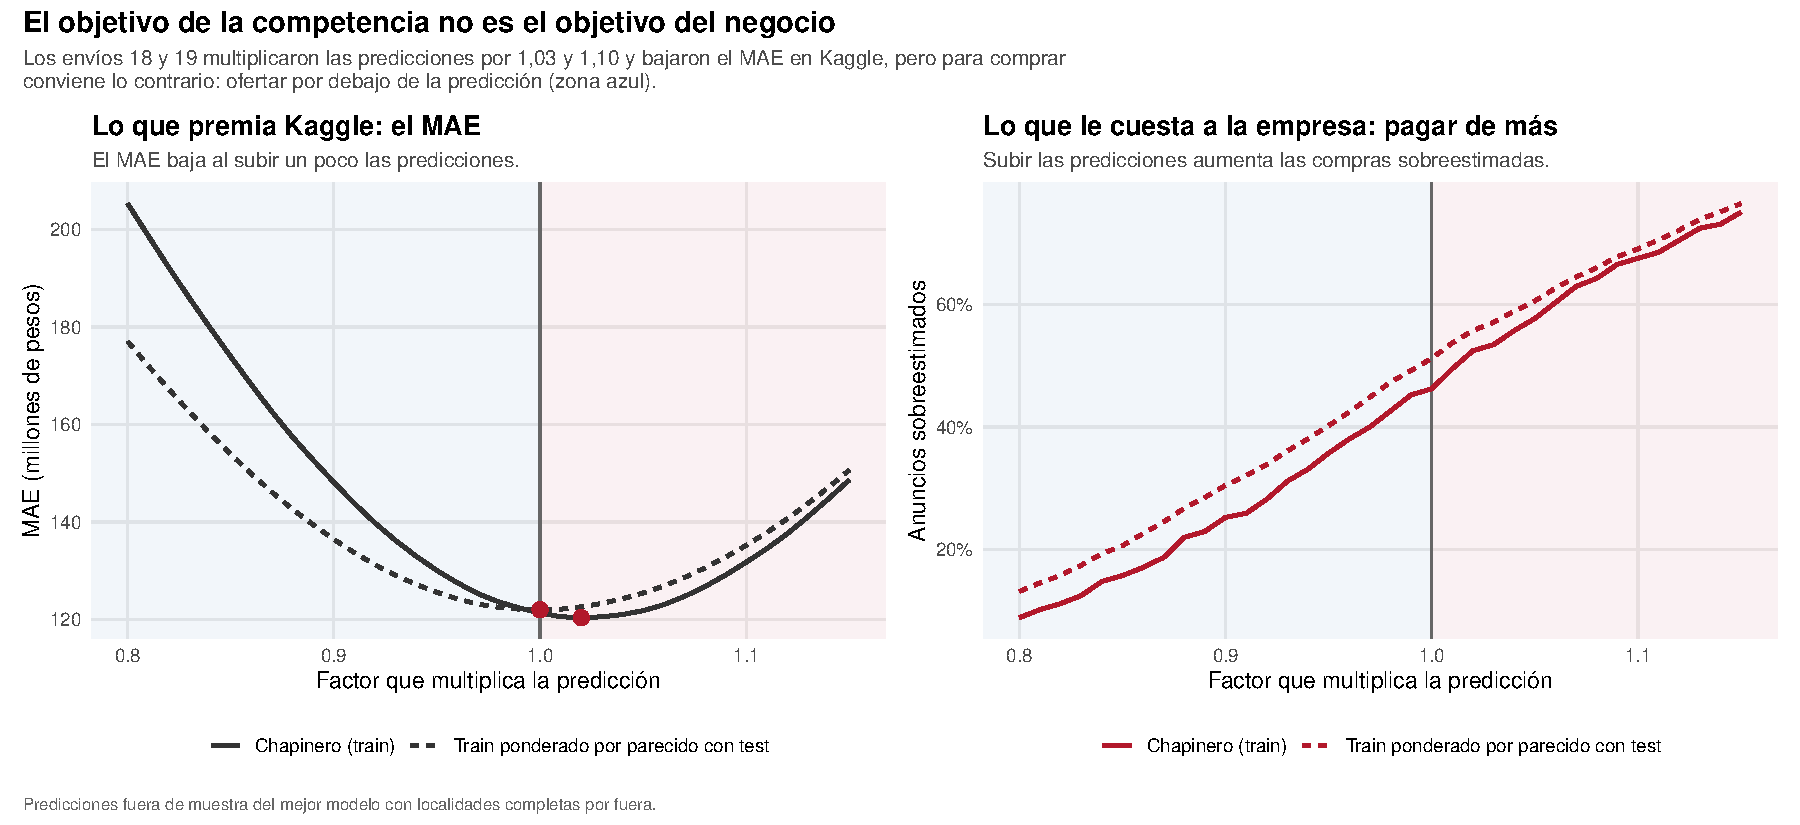
\includegraphics[width=\textwidth]{negocio_05_kaggle_vs_negocio.pdf}
  \note{El modelo subestima Chapinero, así que subir un poco las predicciones bajó el MAE en Kaggle. Pero para la empresa es al revés: sobreestimar significa pagar de más y destruir capital, como le pasó a Zillow; subestimar solo hace perder el negocio. La empresa debe ofertar por debajo de la predicción.}
\end{frame}
